\hypertarget{bg-disorder-and-localisation}{%
\section{Disorder and Localisation}\label{bg-disorder-and-localisation}}

Disorder is a fact of life for the condensed matter physicist. No sample will ever be completely free of contamination or of structural defects. The classical Drude theory of electron conductivity envisages electrons as scattering off impurities. Hence we would expect the electrical conductivity to be proportional to the mean free path~\autocite{lagendijkFiftyYearsAnderson2009}, decreasing smoothly as the number of defects increases. However, Anderson showed in 1958~\autocite{andersonAbsenceDiffusionCertain1958} that at some critical level of disorder \textbf{all} single particle eigenstates localise. What would later be known as Anderson localisation is characterised by exponentially localised eigenfunctions \(\psi(x) \sim e^{-x/\lambda}\) which cannot contribute to transport processes. The localisation length \(\lambda\) is the typical scale of localised state and can be extracted with transmission matrix methods~\autocite{pendrySymmetryTransportWaves1994}. Anderson localisation provided a different kind of insulator to that of the band insulator.

The Anderson model is about the simplest model of disorder one could imagine \begin{equation}\protect\hypertarget{eq:bg-anderson-model}{}{
H = -t\sum_{\langle jk \rangle} c^\dagger_j c_k + \sum_j V_j c_j^\dagger c_j
}\label{eq:bg-anderson-model}\end{equation}

It is one of non-interacting fermions subject to a disorder potential \(V_j\) drawn uniformly from the interval \([-W,W]\). The discovery of localisation in quantum systems was surprising at the time given the seeming ubiquity of extended Bloch states. Within the Anderson model, all the states localise at the same disorder strength \(W\) but later Mott showed that in other contexts extended Bloch states and localised states could coexist at the same disorder strength but different energies. The transition in energy between localised and extended states is known as a mobility edge~\autocite{mottMetalInsulatorTransitions1978}.

Localisation phenomena are strongly dimension dependent. In three dimensions the scaling theory of localisation~\autocite{edwardsNumericalStudiesLocalization1972,kramerLocalizationTheoryExperiment1993} shows that Anderson localisation is a critical phenomenon with critical exponents both for how the conductivity vanishes with energy when approaching the mobility edge and for how the localisation length increases below it. By contrast, in one dimension disorder generally dominates. Even the weakest disorder exponentially localises \emph{all} single particle eigenstates in the one dimensional Anderson model. Only long-range spatial correlations of the disorder potential can induce delocalisation~\autocite{aubryAnalyticityBreakingAnderson1980,dassarmaLocalizationMobilityEdges1990,dunlapAbsenceLocalizationRandomdimer1990,izrailevLocalizationMobilityEdge1999,croyAndersonLocalization1D2011,izrailevAnomalousLocalizationLowDimensional2012}.

Later localisation was found in disordered interacting many-body systems:

\[
H = -t\sum_{\langle jk \rangle} c^\dagger_j c_k + \sum_j V_j c_j^\dagger c_j + U\sum_{jk} n_j n_k
\] Here, in contrast to the Anderson model, localisation phenomena are robust to weak perturbations of the Hamiltonian. This is called many-body localisation (MBL)~\autocite{imbrieManyBodyLocalizationQuantum2016}.

Both MBL and Anderson localisation depend crucially on the presence of \emph{quenched} disorder. Quenched disorder takes the form a static background field drawn from an arbitrary probability distribution to which the model is coupled. Disorder may also be introduced into the initial state of the system rather than the Hamiltonian. This has led to ongoing interest in the possibility of disorder-free localisation where the disorder is instead \emph{annealed}. In this scenario the disorder necessary to generate localisation is generated entirely from the thermal fluctuations of the model.

The concept of disorder-free localisation was first proposed in the context of Helium mixtures~\autocite{kagan1984localization} and then extended to heavy-light mixtures in which multiple species with large mass ratios interact. The idea is that the heavier particles act as an effective disorder potential for the lighter ones, inducing localisation. Two such models~\autocite{yaoQuasiManyBodyLocalizationTranslationInvariant2016,schiulazDynamicsManybodyLocalized2015} instead find that the models thermalise exponentially slowly in system size, which Ref.~\autocite{yaoQuasiManyBodyLocalizationTranslationInvariant2016} dubs Quasi-MBL.

True disorder-free localisation does occur in exactly solvable models with extensively many conserved quantities~\autocite{smithDisorderFreeLocalization2017}. As conserved quantities have no time dynamics this can be thought of as taking the separation of timescales to the infinite limit. The localisation phenomena present in the Falikov-Kimball model are instead the result of annealed disorder. A strong separation of timescales means that the heavy species is approximated as immobile with respect to the lighter itinerant species. At finite temperature the heavy species acts as a disorder potential for the lighter one. However, in contract to quenched disorder, the probability distribution of annealed disorder is entirely determined by the thermodynamics of the Hamiltonian. In the two dimensional FK model this leads to multiple phases where localisation effects are relevant. At low temperatures the heavy species orders leading to a traditional band gap insulator. At higher temperatures however thermal disorder causes the light species to localise. At weak coupling, the localisation length can be very large, so finite sized systems may still conduct, an effect known as weak localisation~\autocite{antipovInteractionTunedAndersonMott2016}.

In Chapter 3 we will consider a generalised FK model in one dimension and how the disorder generated near a one dimensional thermodynamic phase transition interacts with localisation physics.

So far we have considered disorder as a static or dynamic field coupled to a model defined on a translation invariant lattice. Another kind of disordered system that worthy of study are amorphous systems.

Amorphous systems have disordered bond connectivity, so called \emph{topological disorder}. As discussed in the introduction these include amorphous semiconductors such as amorphous Germanium and Silicon ~\autocite{Yonezawa1983,zallen2008physics,Weaire1971,betteridge1973possible}. While materials do not have long range lattice structure they can enforce local constraints such as the approximate coordination number \(z = 4\) of silicon.

Topological disorder can be qualitatively different from other disordered systems. Disordered graphs are constrained by fixed coordination number and the Euler equation. The Harris~\autocite{harrisEffectRandomDefects1974} and the Imry-Mar~\autocite{imryRandomFieldInstabilityOrdered1975} criteria are key results on the effect of disorder on thermodynamic phase transitions. The Harris criterion signals when disorder will affect the universal of a thermodynamic critical point. It states that for a critical point in a \(d\)-dimensional system with correlation length scaling exponent, disorder will be relevant if \(\nu\) if \(d\nu < 2\). The Imry-Ma criterion simply forbids the formation of long range ordered states in \(d \leq 2\) dimensions in the presence of disorder. The latter criteria is violated in the presence of correlated disorder~\autocite{changlaniChargeDensityWaves2016} and both are modified for topological disorder. In chapter 4 we will put the Kitaev model onto two dimensional Voronoi lattices. These lattices are have fixed coordination number \(z=3\) and must satisfy the Euler equation for the plane, this leads to strong anti-correlations which mean that topological disorder is effectively weaker than standard disorder here~\autocite{barghathiPhaseTransitionsRandom2014,schrauthViolationHarrisBarghathiVojtaCriterion2018}{]}. This does not apply to the three dimensional Voronoi lattices where the Euler equation is a weaker constraint.

Lastly it is worth exploring how quantum spin liquids and disorder interact. The KH model has been studied subject to both flux \autocite{Nasu_Thermal_2015} and bond \autocite{knolle_dynamics_2016} disorder. In some instances it seems that disorder can even promote the formation of a QSL ground state~\autocite{wenDisorderedRouteCoulomb2017}. I will look at how adding lattice disorder to the mix affects the picture. It has also been shown that the KH model exhibits disorder free localisation after a quantum quench~\autocite{zhuSubdiffusiveDynamicsCritical2021}.

\hypertarget{diagnosing-localisation-in-practice}{%
\subsection{Diagnosing Localisation in practice}\label{diagnosing-localisation-in-practice}}

\hypertarget{fig:localisation_radius_vs_length}{%
\begin{figure}
\centering
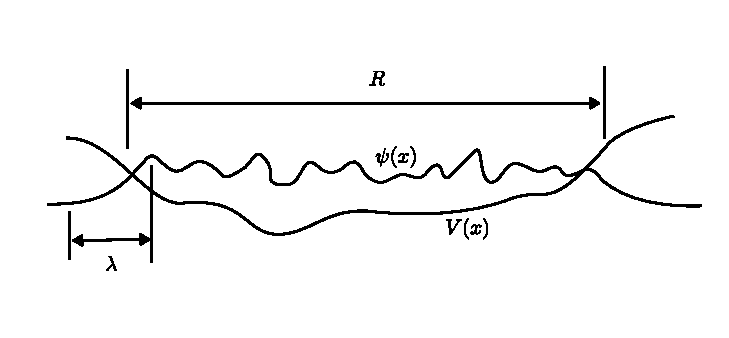
\includegraphics[width=1\textwidth,height=\textheight]{figure_code/background_chapter/localisation_radius_vs_length}
\caption[{Localisation length vs diameter}]{A localised state \(\psi\) in an potential well that has formed from random fluctuations in the disorder potential \(V(x)\). The localisation length \(\lambda\) governs how quickly the state decays away from the well while the diameter \(R\) of the state is controlled by the size of the well. Reproduced from~\autocite{kramerLocalizationTheoryExperiment1993}.}
\label{fig:localisation_radius_vs_length}
\end{figure}
}

Looking at practical tools for diagnosing localisation, there are a few standard methods~\autocite{kramerLocalizationTheoryExperiment1993}.

The most direct method would be to fit a function of the form \(\psi(x) = f(x) e^{-|x-x_0|/\lambda}\) to each single particle wavefunction to extract the localisation length \(\lambda\). This method is little used in practice since it requires storing and processing full wavefunctions which quickly becomes expensive for large systems.

For low dimensional systems with quenched disorder, transmission matrix methods can be used to directly extract the localisation length. These work by turning the time independent Schrödinger equation \(\hat{H}|\psi\rangle = E|\psi\rangle\) into a matrix equation linking the amplitude of \(\psi\) on each \(d-1\) dimensional slice of the system to the next and looking at average properties of this transmission matrix. This method is less useful for systems like the FK model where the disorder as a whole must be sampled from the thermodynamic ensemble. It is also problematic for the Kitaev Model on an amorphous lattice as the slicing procedure is complex to define in the absence of a regular lattice.

A more versatile method is based on the inverse participation ratio. The inverse participation ratio is defined for a normalised wave function \(\psi_i = \psi(x_i), \sum_i |\psi_i|^2 = 1\) as its fourth moment~\autocite{kramerLocalizationTheoryExperiment1993}:

\[
P^{-1} = \sum_i |\psi_i|^4
\]

The name derive from the fact that this operator acts as a measure of the volume where the wavefunction is significantly different from zero. They can alternatively be thougt of as providing a measure of the average diameter \(R\) from \(R = P^{1/d}\), see \cref{fig:localisation_radius_vs_length} for the distinction between \(R\) and \(\lambda\).

For localised states, the \emph{inverse} participation ratio \(P^{-1}\) is independent of system size while for plane wave states in \(d\) dimensions \(P^{-1} = L^{-d}\). States may also be intermediate between localised and extended, described by their fractal dimensionality \(d > d* > 0\):

\[
P(L)^{-1} \sim L^{-d*} 
\]

For finite size systems, these relations only hold once the system size \(L\) is much greater than the localisation length. When the localisation length is comparable to the system size the states contribute to transport. This is called weak localisation~\autocite{altshulerMagnetoresistanceHallEffect1980,dattaElectronicTransportMesoscopic1995}.

For extended states \(d* = 0\) while for localised ones \(d* = 0\). In both chapters I will use an energy resolved IPR \[
DOS(\omega) = \sum_n \delta(\omega - \epsilon_n)\\
IPR(\omega) = DOS(\omega)^{-1} \sum_{n,i} \delta(\omega - \epsilon_n) |\psi_{n,i}|^4
\] Where \(\psi_{n,i}\) is the wavefunction corresponding to the energy \(\epsilon_n\) at the ith site. In practice I bin the energies and IPRs into a fine energy grid and use the mean within each bin.
